%\documentclass{cumcmthesis} 这里面是承诺书 
\documentclass[withoutpreface,bwprint]{cumcmthesis} 
\usepackage{ctex} % 支持中文
\usepackage{booktabs} % 支持三线表
\usepackage{geometry} % 支持页面布局
\usepackage[framemethod=TikZ]{mdframed}
\usepackage{url}   % 网页链接
\usepackage{subcaption} % 子标题
\usepackage{booktabs}
\usepackage{threeparttable}
\usepackage{svg}
\usepackage{graphicx}
\geometry{a4paper,scale=0.8} % 设置页面布局为A4纸,缩放比例为0.8

\title{基于XXX的XXX研究}
\tihao{C}
\baominghao{xxxx}
\schoolname{XMUM}
\membera{Liang Zimao}
\memberb{Wang Ziwen}
\memberc{Jiang Yecen}
\supervisor{  }
\yearinput{2024}
\monthinput{09}
\dayinput{08}

\begin{document}

\maketitle

\keywords{\textbf{0-1整数规划}\quad \textbf{动态规划} \quad \textbf{单边检验} \quad \textbf{概率统计分析}}

\section{摘要}
摘要内容

\section{问题重述}
\subsection{问题背景}
在竞争激烈的现代制造业中,产品质量是企业立足市场的关键。面对市场对电子产品等高科技领域产品质量的日益严苛要求,企业必须在确保产品性能和可靠性的同时,有效控制成本。这要求企业在采购、检测、组装及处理不合格品等生产环节做出明智的决策。

产品质量的保障始于零配件的质量控制。在成本压力下,企业需在检测频率、成本和产品质量间找到平衡点。此外,不合格产品不仅损失产品价值,还会影响品牌信誉和客户满意度,增加售后服务成本。因此,企业的决策需综合考虑直接成本和潜在的市场风险。
数学建模为解决这一挑战提供了有力的工具,通过量化分析生产过程中的各种因素,帮助企业在保证产品质量的同时,实现成本最优化。

\subsection{问题重述}
问题一:供应商声称一批零配件的次品率不会超过某个标称值。需要设计一个抽样检测方案,以最少的检测次数确定是否接收这批零配件。假设标称值为10\%,需要针对两种情形给出具体结果:在95\%的信度下拒收次品率超过标称值的零配件;在90\%的信度下接收次品率不超过标称值的零配件。

问题二:结合已知两种零配件和成品的次品率,为生产过程的各个阶段制定决策方案以实现成本控制。决策包括是否检测零配件、是否检测成品、是否拆解不合格成品。

问题三:对包含多道工序和多个零配件的生产过程制定新的整体的生产策略,以实现成本控制。

问题四:假设问题2和问题3中的次品率数据是通过抽样检测方法得到的,重新评估和优化问题二、三生产过程中的决策。

\section{问题分析}
\subsection{问题一}


\subsection{问题二}
问题二是对生产-包装流程的最优处理策略,旨在最小化企业生产总成本。本质是一个0-1整数规划问题,因此应首先确定决策变量,即是否对零配件1、零配件2和成品进行检测,以及是否对不合格成品进行拆解。这些决策变量将直接影响生产成本和利润。接下来根据题目提供的数据,构建目标函数。目标是最大化利润。由于在本问题中,所有可能性仅有 6 $\times 2^{4}$ =96种,因此出于简化问题的考虑采用穷举法来得出所有情况,并求出最优决策

\subsection{问题三}
问题三分析。

\subsection{问题四}
问题四分析

\section{模型假设}
\begin{itemize}
    \item 市场需求无限大,生产出的成品可以被全部卖出。
\end{itemize}





\section{变量说明}
\begin{table}[htbp]
    \centering
    \begin{threeparttable}
    \caption{变量说明表}
    \begin{tabular}{ccc}
        \toprule
        符号 & 含义 & 单位 \\
        \midrule
        占位 & 占位 & 占位 \\
        占位 & 占位 & 占位 \\
        占位 & 占位 & 占位 \\
        占位占位占位占位 & 占位占位占位占位占位 & 占位占位占位占位占位 \\
        \bottomrule
    \end{tabular}
    \begin{tablenotes}
        \item 注:未列出的符号以及重复出现的符号以出现处为准
    \end{tablenotes}
    \end{threeparttable}
\end{table}

\section{模型建立与求解}
\subsection{问题一模型求解}

\subsection{问题二模型建立}
问题二中,企业在生产过程中需要在多个阶段做出决策,包括是否对零配件进行检测、是否对成品进行检测,以及是否对不合格的成品进行拆解。以下是对这些决策的逻辑重构和详细分析:

成本效益模型
为了优化生产过程,企业需要最小化总成本,这可以通过成本效益分析模型来实现。总成本由以下几部分组成:
\begin{itemize}
    \item 装配成本:将零配件装配成完整成品所需的成本
    \item 检测成本:检测零配件或者成品所需的成本
    \item 拆解成本:对检验出不合格的成品进行拆解所需的成本
    \item 调换成本:调换进入市场的不合格成品的损失(包括隐形损失)
    \item 销售收益:卖出成品的收益
\end{itemize}

\subsubsection{装配的成本决策:}
企业需要装配成品,每装配一次,成本为:$C_{\text{单件装配}}$
由于企业装配

\subsubsection{零配件检测的成本决策:}
企业需要决定是否对零配件进行检测。如果选择检测,不合格的零配件将被丢弃;不检测则将直接用于装配。检测成本和不检测可能导致的损失:

检测成本:$C_{\text{检测}} = n \times C_{\text{单件检测}}$

不检测的损失(潜在) :$C_{\text{损失}} = n \times p_1 \times C_{\text{装配损失}} + C_{\text{调换损失}}$

如果检测成本低于不检测成本($C_{\text{检测}}<C_{\text{损失}}$),选择检测;反之则选择不检测。

\subsubsection{成品检测的成本决策:}
企业同样需要决定是否对成品进行检测,若不检测,则不合格的成品有可能进入

成品检测成本:$C_{\text{成品检测}} = m \times C_{\text{单件成品检测}}$

不检测的损失(潜在):$C_{\text{调换损失}} = m \times p_{\text{成品}} \times C_{\text{调换}}$

如果检测成本低于不检测成本($C_{\text{成品检测}}<C_{\text{调换}}$),选择检测;反之则选择不检测。

\subsubsection{不合格成品拆解的成本决策}
对于检测出的不合格成品,企业可以选择拆解以回收可用的零配件或直接丢弃。拆解成本和拆解收益之差是决策的关键:

拆解成本:$C_{\text{拆解}} = k \times C_{\text{单件拆解}}$ 

拆解收益:$C_{\text{拆解收益}} = k \times p_{\text{合格零件}} \times C_{\text{零件回收}}$

\subsubsection{综合决策模型}

综合考虑所有阶段的成本和收益,构建总成本模型,以确定是否进行检测或拆解,优化生产流程的成本结构
总成本

$$C_{\text{总}} = min(\sum (C_{\text{零件检测}} + C_{\text{装配}} + C_{\text{成品检测}} + C_{\text{拆解}}))$$


\subsection{问题二模型求解}

\begin{figure}[htbp]
    \centering
    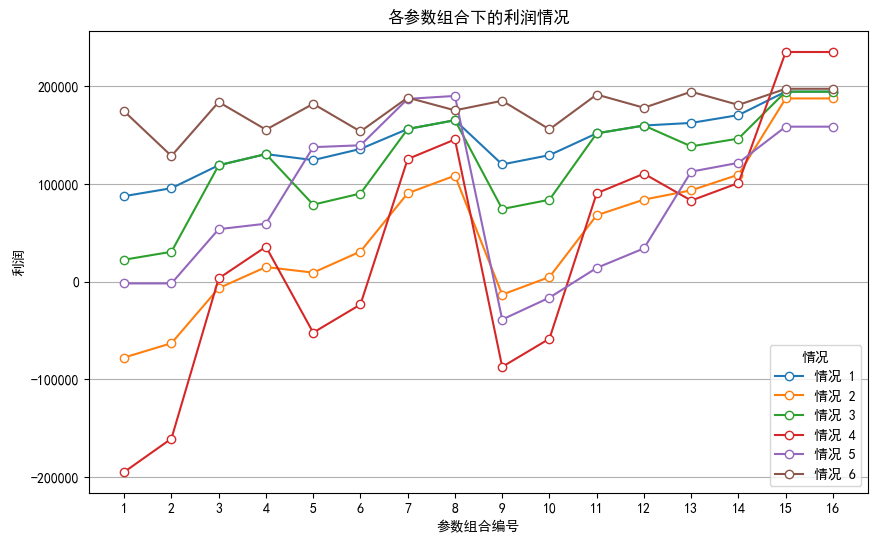
\includegraphics[width=1\linewidth]{figure/各参数组合的利润情况.png}
    \caption{各参数组合下的利润情况}
    \label{profit}
\end{figure}




\subsection{问题三模型建立}

\subsection{问题三模型求解}

\subsection{问题四模型建立}

\subsection{问题四模型求解}


\section{模型分析与检验}
模型分析与检验内容。

\section{模型评价与改进}
模型评价与改进内容。

\section{参考文献}
参考文献内容。

\section{附录}
附录内容。

\end{document}

